\section{The $t-V$ Model}
\label{sec:t-VIntro}

So called "toy models" are ubiquitous in condensed matter physics. These describe a complex system in simple terms so that attention can be given to an underlying mechanism of such system. The Ising model, in it simplest form, can describe how a system spontaneously becomes a ferromagnet by considering interactions between quantum spins and tuning an external temperature. Similarly, the Hubbard model considers the interaction strength of electrons on a lattice and a hopping rate to describe the transition between conductor and insulator. The fact that the two aforementioned examples mention phase transitions is not mere coincidence. 

Near a phase transition, evidence seems to point out to the fact that the behavior of a system is determine by a small set of parameters, a phenomenon known as universality. The size of a lattice could be one of these parameters, perhaps it could be the number of elements, or maybe even symmetry properties. Different systems having the same value for such universality parameters are said to fall under the same universality class. 

The studies that will be presented in this thesis shall be concerned with a specific model, which shall be referred to as the $t-V$ model. This model, is mapped from the $XXZ$ spin model and describes $N$ itinerant fermions on a 1D lattice of size $L$. These fermions can tunnel to neighboring sites and the rate at which they do so is proportional to a hopping parameter $t$. An interaction potential, $V$, between the fermions is also considered, which could be repulsive ($V > 0$) or attractive ($V < 0$). Periodic and anti-periodic boundary conditions will be assumed for the case of odd and even particles, respectively. Mathematically, this is represented by the following Hamiltonian:
%
\begin{equation}
H = -t \sum_{i} \left ( c_{i}^{\dag} c_{i+1} + c_{i+1}^{\dag} c_{i} \right )+ V \sum_{i} n_i n_{i+1}   
\label{eq:t-VHamiltonian}
\end{equation}
%
where $c_{i}^{\dag}$ ($c_{i}$) creates (annihilates) a fermion on site $i$ and $n_{i}$ counts the number of fermions on site $i$. In the case that there exists a fermion on site $i$ already, then $c_{i}^{\dag} = 0$ in order to satisfy Pauli's Exclusion Principle. The interaction term can then be understood conceptually as adding to the potential energy of the system if there are multiple particles in neighboring sites. Conceptually, the first term may be more difficult to understand in its current representation, due to this operator being non-diagonal. Nevertheless, expressing it in the momentum basis, which is diagonal, will illustrate that how contributions to the kinetic energy will come from all particles with nonzero momentum (which will be all of them unless $t=0$). A detailed mapping of the kinetic energy operator from lattice site to momentum basis can be seen in Appendix \ref{appendix:kineticMapping}.

test Eq.~(\ref{eq:t-VHamiltonian})

%%%%%%%%%%%%%%%%%%%
\begin{figure*}[thp]
\begin{center}
\includegraphics[width=1.0\textwidth]{phaseDiagramtV.pdf}
\end{center}
\caption{Phase diagram of the $t-V$ model accompanied by pictures of candidate ground states for $N=2$ fermions on a $L=4$ site lattice. For the purposes of measuring accessible entanglement, the lattice has been bipartitioned into spatial subregions $A$ (blue) and $B$ (red), each of size $\ell = 2$. We assume periodic boundary conditions. In the limit of strong attractive interactions where $V/t \ll -2$, the particles cluster together and there are $L$ equally probable configurations corresponding to all translations of the cluster.  At the first order phase transition where $V/t = -2$, all ${L}\choose{N}$ configurations are equally probable resulting in a flat state. In the TLL phase with $|V/t| < 2$,  particles are delocalized and we have included a characteristic state corresponding to free fermions $(V=0)$. In the limit of strong repulsive interactions where $V/t \gg 2$, fermions maximize their distance from each other resulting in a charge density wave (CDW) phase. The open and closed circles on the $V/t$ axis denote a first order and continuous phase transition, respectively.}
\label{fig:phaseDiagram}
\end{figure*}
%%%%%%%%%%%%%%%%%

Figure \ref{fig:phaseDiagram} shows the phase diagram of the $t-V$ model. For $V/t \ll -2$, the fermions cluster together due to the strong attractive interaction. The state in this regime is an equal superposition of all possible such cluster configurations over all lattice sites. At $V/t = -2$, the system undergoes a second order phase transition into the Tomonaga-Luttinger Liquid (TLL) phase. Here, the state is in a superposition of all possible configurations of the fermions on the lattice. The weights for these configurations are in general different and can only be exactly known at $V/t = 0$ \cite{PhysRevLett.121.150501}. At $V/t = 2$, the system undergoes a continuous phase transition into the charged density wave (CDW) phase. At $V/t \gg 2$, the strong repulsion between particles leads to them forming an alternating pattern of particle-vacancy-particle-vacancy \dots The state in this regime becomes an equal superposition of the only two possible such configurations.

Notice that in Figure \ref{fig:phaseDiagram} the lattice sites have two different colors, blue and red. This is to illustrate that a system can be partitioned into smaller subregions. In this particular example, each partition would be of size 2 lattice sites. In fact, subdividing a system into this smaller subsystems will be necessary for the main phenomenon of interest in this thesis: quantum entanglement. The bulk of this work will consist on quantifying the amount of entanglement of a system via entropy measures. Before getting to explaining entanglement, in the next section, an overview of entropy or information measures will be given.

\section{Information measures}
\label{sec:informationMeasures}

	The probabilistic nature of quantum mechanics, provides an ideal test bed for entropy measures. In section \ref{sec:t-VIntro}, it was mentioned that knowing something about $A$, will give you information about its entangled pair $B$. The amount of information gained in such measurement can be quantified by the entropy of the system. Recall that, in essence, entropy is a measure directly proportional to the disorder of a system. Thus, doing a measurement on a high entropy state, will give more information than in a highly ordered state, in which the outcome of the measurement is more like to be known a priori. For this reason, these will be referred to as information of this work for the remainder of this work.
	
	In this section, the information measure from which the ones that will be used to quantify entanglement will be introduced. Then, the actual measures of entanglement will be presented.
	
	\subsection{Shannon entropy}
	
	The Shannon or information entropy is the average amount of information gained from a a data set in which the entries occur according to some probability distribution. It is defined as:
	%
	\begin{equation}
	S = -\sum_{i} p_i \log_{b} p_i
	\label{eq:shannonEntropy}
	\end{equation}
	%
	where the sum is carried over all entries in the data set and $p_i$ is the probability of measuring entry $i$. The base $b$ can be chosen arbitrarily depending on the context. The base will be chosen as the number $e$ such that $\log_b \to \ln$ for the remainder of this work. Up next, a common day example will be presented in order to give some intuition about how information gain can be estimated with Eq.~\eqref{eq:shannonEntropy}
	
	Consider a regular coin flip. Disregarding all physical effects that can somehow bias the outcome, it is expected that either heads or tails will randomly be with equal probability $1/2$. Then, since there is no bias towards any of the two possible outcomes of the coin flip, the information gain should be at a maximum. The Shannon entropy for this case is:
	%
	\begin{align}
	S &= -\frac{1}{2} \ln{\frac{1}{2}} - \frac{1}{2} \ln{\frac{1}{2}}  \nonumber\\
	&= \ln{2}  \nonumber \\
	S &\approx 0.6931 \nonumber \dots
	\end{align}
	Now, consider a coin that has been modified in such a way that it is more likely to get one outcome than the other. For the sake of this example, let's say that heads shall occur with probability $2/3$, while tails with $1/3$. Then, since it is two times more likely that heads will occur instead of tails, more certainty about the outcome is known beforehand and thus the information gained decreases. Shannon entropy gives:
	%
	\begin{align}
	S &= -\frac{2}{3} \ln{\frac{2}{3}} - \frac{1}{3} \ln{\frac{1}{3}} \nonumber \\
	S &\approx 0.6365 \dots \nonumber
	\end{align}
	%
	Finally, an extreme case would be a coin that was incorrectly manufactured and has heads on two sides. Opposite to a regular coin, in which maximum information is gained because both heads and tails have the same probability, the probability for heads to land in this case is 1, while 0 for tails. Since the result is already known before the coin flip, the information gain after the coin flip is none. Shannon entropy gives:
	%
	\begin{align}
	S &= -1\ln{1} = 0 \nonumber
	\end{align}
	%	

	Now that some intuitive examples were discussed, the quantum information theory counterpart of Shannon's entropy will be presented.
	
	\subsection{von Neumann entropy}
	
	In calculating the Shannon entropy, the probabilities of random events occurring are required. In quantum mechanics, the state of a system is in general not exactly known and only the probabilities of measuring a state are known. The probabilities of finding a system in a certain state can be encoded in its density matrix. The density matrix is defined as:	
	%
	\begin{align}
	\label{eq:densityMatrix}
	\rho = \vert \Psi \rangle \langle \Psi \vert
	\end{align}
	%
	where $\vert\Psi\rangle$ is the state of the full system, such that $\vert \Psi \rangle \in \mathcal{H} = A \otimes B$ and the normalization condition on the states of the system imply that $\Tr \rho = 1$. The state $\vert \Psi \rangle$ can be partitioned into subregions or subsystems that live in Hilbert Space $A$ and $B$, respectively. The von Neumann entropy measures the information gained about subsystem $B$ by doing a measurement on subsystem $A$. The von Neumann entropy is defined as:
	%
	\begin{equation}
	S = -\Tr\rho_{A} \ln{\rho_A}
	\label{eq:vonNeumannEntropy}
	\end{equation}
	%
	where $\rho_A$ is known as the reduced density matrix of subsystem $A$ and it is obtained by tracing out the degrees of freedom in $B$, an operation known as the partial trace (with respect to $B$, in this case). The reduced matrix of $A$ is then:
	%
	\begin{equation}
	\rho_{A} = \Tr_B \rho = \sum_b \langle \psi_b \vert \Psi \vert \psi_b \rangle
	\label{eq:partialTrace}
	\end{equation}
	%
	where the sum is carried over all possible states in which subsystem $B$ can be in and $\psi_b$ denotes each of these states. Normalization implies that $\Tr \rho_A = 1$.
	
	The von Neumann entropy serves its purpose well, but it relies on having access to the density matrix of the system. Obtaining the density matrix is feasible in one-dimensional systems via exact diagonalization of the ground state Hamiltonian (see Appendix \ref{app:lanczos} for details on exact diagonalization via Lanczos algorithm). But for systems of higher dimensionality, exact diagonalization is out of the picture due to the exorbitant amount of memory required and quantum Monte Carlo (QMC) methods must be employed. In QMC methods, there is no access to the reduced density matrix, but the expectation value of a unitary operator that swaps the $A$ states between two identical copies of a system gives higher powers of the reduced density matrix \cite{Hastings:2010dc}. In other words, $\rho_{A}$ is not accessible but $\rho_{A}^{\alpha}$ can be obtained for $\alpha > 1$. It was also shown experimentally \cite{Islam:2015cm}  that $\rho_A^{\alpha}$ can be obtained by interference of two identical copies of ultra-cold atoms. Thus, a new formulation of the entropy must be introduced that depends on higher powers of $\rho$.
	
	\subsection{R\'enyi entanglement entropy}
	
	In order to calculate entropy via QMC or experimentally, a measure that depends on powers of the reduced density matrix larger than 1 must be used, since these methods do not have access to the reduced density matrix. The R\'enyi entanglement entropy, which is the analogue of the R\'enyi entropy from information theory, provides an information measure that depends on $\rho_{A}^{\alpha}$ instead of $\rho_{A}$. The R\'enyi entanglement entropy is defined as:
	%	
	\begin{equation}
	\label{eq: renyiEE}
	S_{\alpha} = \frac{1}{1-\alpha} \ln \Tr \rho_{A}^{\alpha}
	\end{equation}
	%
	where $\alpha$ is known as the R\'enyi index. In the limit of $\alpha \to 1$, the R\'enyi entanglement entropy becomes to the von Neumann entropy. Higher R\'enyi indices will result in lower R\'enyi entanglement entropies, as shall be discussed up next.
	
	Due to the normalization conditioned imposed on the reduced density matrix, the sum of its eigenvalues must also be unity. Each of the eigenvalues must then belong to the closed interval $\left [ 0,1 \right ]$. Raising $\rho_A$ to a power $\alpha > 1$ is equivalent to raising each eigenvalue by $\alpha$ and as a result, the trace of $\rho_A$ will decrease. A lower trace of $\rho_A$ will then make the R\'enyi entanglement entropy lower. Thus, $S_{\alpha}$ is a monotonically decreasing function of $\alpha$. 
	
	Now that the $t-V$ model and the information measures have been introduced, it is time to discuss quantum entanglement itself.
	
\section{Quantum entanglement}
\label{sec:quantumEntanglement}

	A quantum many body system is entangled if its constituents present correlations that cannot be classically described. In other words, assuming subsystems $A$ and $B$ are entangled with one another, knowing something about $A$ automatically gives you some knowledge of $B$. 	Mathematically, a quantum many-body system is entangled if it cannot be factored into a tensor product of the state of subsystems $A$ and $B$. The condition for entanglement is then,
%	
	\begin{equation}
	\vert\Psi\rangle \neq \vert\Psi_{A}\rangle \otimes \vert\Psi_{B}\rangle
	\label{eq:entanglementCondition}
	\end{equation}
%
	Since the average information gained about $B$ when measuring $A$ can be quantified via von Neumann and R\'enyi entanglement entropies, these can be used as indication of how entangled the two subsystems are with each other. A system is highly entangled if its state possesses a large entanglement entropy.
	
	The subsystems in which a system is partitioned can represent subsets of particles or quantum modes. The modes can represent spatial subregions, momenta, spins, etc... Since the case of entanglement in the $t-V$ model under a spatial bipartition was studied in this work, from here onwards, the mode partition shall be referred to as a spatial partition. Up next, an overview of particle-partitioned and spatially-partitioned entanglement is given
	
	A many-body system can be partitioned into subsets of particles. In the case of a particle bipartition, one of the subsets will have $n$ particles and its complementary subset, $N-n$ particles, where $N$ is the total number of particles in the system. To quantify entanglement between the subsets of particles, the $n-$body reduced density matrix ($n-RDM$) is used:
	%
	\begin{equation}
	\rho_{n} = \int dx_{n+1} \dots \int dx_N \langle x_{n+1} \dots x_N \vert\Psi\rangle \langle\Psi\vert x_{n+1} \dots x_N \rangle
	\label{eq:nBodyDensityMatrix}
	\end{equation}
	%
	where $\vert\Psi\rangle$ is the first quantized wavefunction of a system of $N$ identical particles and it properly anti-symmetrized or symmetrized for fermions and bosons, respectively.  The entanglement of a system under a particle bipartition allows to measure non-local effects, complementing the study of spatial entanglement. 
	In measuring spatial entanglement, a system is bipartitioned into a spatial subregion of size $\ell_{A}$ and a complementary region size $L - \ell_A \equiv \ell_B$. Under this type of partition, states are represented in second quantization. In other words, a state $\vert\Psi\rangle = \vert n_1 \rangle \otimes \vert n_2 \rangle \dots \otimes \vert n_N \rangle$ is characterized by the set of occupation numbers on each site. Figure \ref{fig:spatialParticle} illustrates schematically a $1D$ lattice of size $L = 7$ and $N = 3$ under a spatial and then a particle bipartition.
	%%%%%%%%%%%%%%%%%%%
\begin{figure*}[thp]
\begin{center}
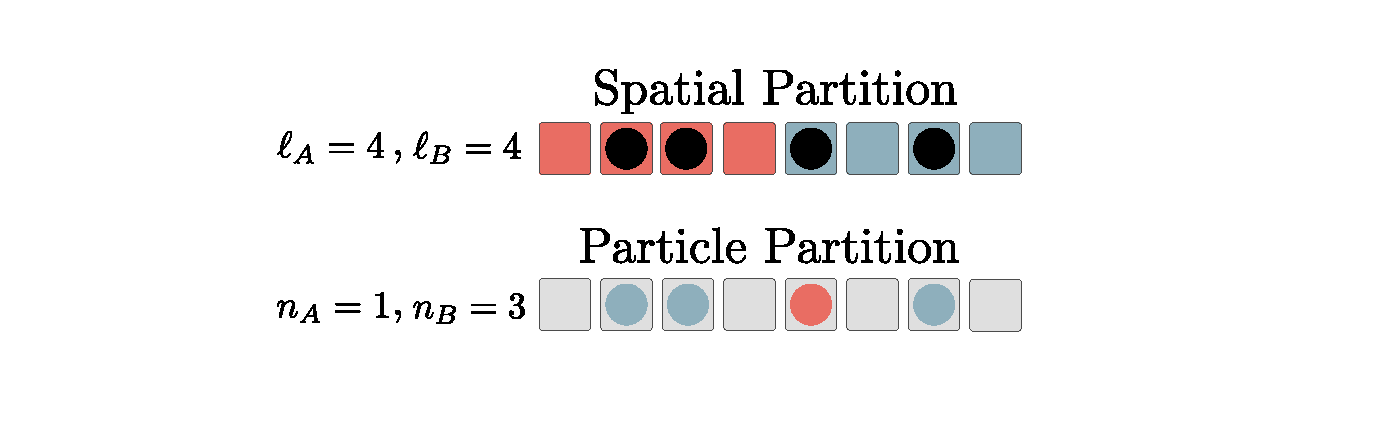
\includegraphics[width=1.0\textwidth]{spatialParticle.pdf}
\end{center}
\caption{Schematic of a one-dimensional lattice of $L=7$ sites and $N=3$ particles under two types of bipartitions. The top lattice is bipartitioned into two spatial subregions $A$ (red) and $B$ (blue). The size of subregion is $\ell_A = 4$ sites, while $\ell_B = L - \ell_A = 3$. The bottom lattice is bipartitioned into two subsets of identical particles. Subset $A$ consists of only of $n_A=1$ particle, while $B$ consists of $n_B = N - n = 2$.}
\label{fig:spatialParticle}
\end{figure*}
%%%%%%%%%%%%%%%%%	
	
	\subsection{Accessible Entanglement}
	Whether it's under a particle or spatial bipartition, the goal is to use the entanglement present in a system as a resource. The von Neumann and R\'enyi entropies give a good mathematical understanding of the entanglement of a system. Nevertheless, for physical applications, conservation laws, such as total particle number and spin must be considered. In Ref.~\cite{Wiseman:2003jx}, a new formulation for the entanglement was proposed that takes such conservation laws, or super selection rules (SSR) into account. 
	
	For a quantum many-body system subject to physical laws conserving some quantity (particle number, charge, spin, etc.), the set of local operations on the state $\ket{\Psi}$ are limited to those that don't violate the corresponding global superselection rule.  For simplicity, attention will be focused to the case of fixed total particles $N$ and thus we are restricted to only those operators which locally preserve the particle number in $A$.  The effect this has on the amount of entanglement that can be transferred to a qubit register is apparent from the simple example (adapted from Ref.~\cite{Wiseman:2003jx} of one particle confined to two spatial modes $A$ and $B$ corresponding to site occupations.  Then, for the state $\ket{\Psi} = \left(\ket{1}_A \otimes \ket{0}_{B} + \ket{0}_A \otimes \ket{1}_{B} \right)/\sqrt{2}$, Eq.~\eqref{eq:vonNeumannEntropy} gives that $S_1 = \ln 2$. However, this entanglement cannot be transferred to a register prepared in initial state $\ket{0}_R$ via a $\texttt{SWAP}$ gate:
\begin{align*}
    & \texttt{SWAP} \ket{0}_R\otimes\left(\ket{1}_A \otimes
    \ket{0}_{B} + \ket{0}_A \otimes \ket{1}_{B} \right)/\sqrt{2} \\
    &= \frac{1}{\sqrt{2}}\left( \ket{0}_R \otimes \underbrace{\ket{0}_A \otimes
        \ket{1}_{B}}_{N=1} + \ket{1}_R \otimes \underbrace{\ket{0}_A \otimes
    \ket{0}_{B}}_{N\neq1} \right)
    % &= \frac{1}{\sqrt{2}}\ket{0}_R \otimes \ket{0}_A \otimes
    %     \ket{1}_{B}
\end{align*}
Notice that the first term post $\texttt{SWAP}$ preserves particle number in the resource, since there is a total of 1 particle in $A$ and $B$. But, last term is not physically allowed since it has no particles at all in $A$ and $B$, thus violating the restriction that total particle number be fixed. The state of the register post-swap will remain in a product state, meaning that the amount of entanglement that can be accessed as a resource is identically zero. In general, it will be seen that the amount of accessible entanglement will be less or equal than the full entanglement of the system.

Formally, the accessible entanglement is defined as:
%
\begin{equation}
\label{eq:accS1}
S_1^{\rm acc} = \sum_n P_n S_1(\rho_{A_{n}})
\end{equation}
%
where the sum is carried over all possible local particle numbers of $A$, $P_n$ is the probability that subsystem $A$ will have $n$ particles, $S_1$ is the von Neumann entropy, which will be a function of $\rho_{A_{n}}$. Notice the additional subscript $n$ in the reduced density matrix expression. Whereas for the full entanglement entropy, knowing $\rho_A$ would suffice, for the accessible entanglement entropy, the reduced density matrix must be also be projected onto the subspace of local particle number $n$. Additionally, recall that the normalization condition asks for $\sum_n P_n = 1$. This accessible entropy was originally only well defined for the von Neumann entropy $S_1$. Recently, a generalized version of the accessible entanglement that works for R\'enyi indices greater than 1 was proposed \cite{Barghathi:2018oe}, such that any accessible R\'enyi entropy can now be calculated.

Now that all the ground work for the results presented in this thesis has been introduced, an outline the remaining chapters is given. In chapter 2, the particle-partitioned entanglement entropies in the $t-V$ model will be studied. Chapter 3 will present computational results that support the generalization of the accessible R\'enyi entropies under spatial bipartitions of the $t-V$ model. Finally, chapter 4 will briefly discuss some unanswered questions that have emerged from the projects presented here and future ones will be discussed.




	

	
